\documentclass[a4paper,11pt]{article}
\usepackage{dmasproject}
% if you need additional LaTeX packages, add them here

\title{A district-wise analysis of COVID-19 in India}
% sort your names alphabetically by last name
\author{
  Debanjan Chatterjee (20111016)
}
\date{September 2020} % change this accordingly

\begin{document}

\maketitle

\begin{abstract}
The ongoing COVID-19 pandemic is affecting everyone around the globe in some way or the other. The global number of COVID-19 cases have reached a staggering amount of over 30 million confirmed cases, with India reaching a total of over 5 million confirmed cases. Large-scale efforts are being made to curb the rate of infection, however various strategies needs to be developed to address the pandemic in India. In this report, a study has been conducted to perform a district-wise analysis of the number of COVID-19 cases in India.
\end{abstract}

\section{Introduction}

Over the past few months, the world has been taken by storm due to an ongoing pandemic. The root cause of the pandemic is the Coronavirus disease-2019 or COVID-19. It is a highly infectious disease caused by severe acute respiratory syndrome corona virus 2 (SARS-CoV-2). It has affected over 200 countries, with a total number of confirmed coronavirus disease cases exceeding 30 million and a devastating number of casualties, almost touching the million mark. India, owing to its large population, has crossed over 5 million confirmed COVID-19 cases, and it is still increasing at an alarming rate. \par

India is a vast and diverse country, the population density varies drastically across various districts. Therefore, it may be a good idea to do a study on the number of confirmed cases across every district. All the data necessary for the district-wise analysis have been collected from \url{https://www.covid19india.org/} using the subsequent APIs available to access the data at \url{ https://api.covid19india.org/}.\par

The first case of COVID-19 in India was detected on 30th January, 2020, in Kerala. Though there have been one or two more cases in the following weeks, our time period of analysis for the study is from 15th, March 2020 to 5th, September 2020.



\section{Result Analysis}

There have been a few interesting findings from the study. While analyzing COVID-19 cases at a district-level, the fairly simple observation is the five districts with the highest number of cases: Pune, Delhi, Mumbai, Bangalore(also known as bengaluru urban), and Thane (ranked high to low). The reason Delhi has been included here despite being a state is because, Delhi along with a few other states, namely Telangana, Manipur, Goa, Assam, Andaman and Nicobar Island, and Sikkim, report confirmed COVID-19 cases at a state level rather than district level.\par

The districts with the lowest number of COVID-19 cases are: Upper Dibang Valley, South West Hills, Kamla, Kra Dadi, Kurung Kumey. Furthermore, using the district-wise data, the average number of cases per state have been calculated. A bar graph with states with the highest state average and the lowest state average has been plotted.\par







\begin{figure}[!tbp]
  \centering
  \begin{minipage}[b]{0.45\textwidth}
    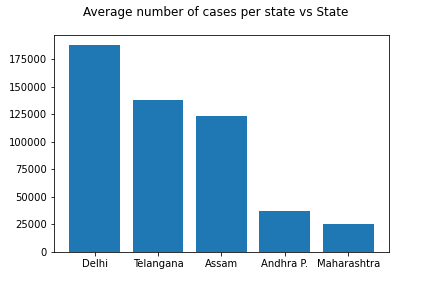
\includegraphics[width=\textwidth]{high-states.png}
    \caption{Five states with highest average}
  \end{minipage}
  \hfill
  \begin{minipage}[b]{0.45\textwidth}
    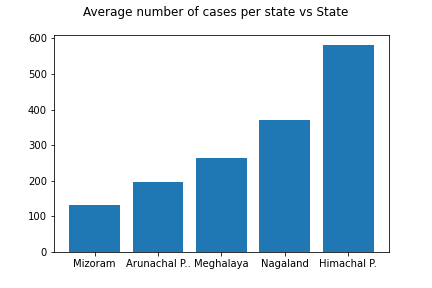
\includegraphics[width=\textwidth]{low-states.png}
    \caption{Five states with the lowest average}
  \end{minipage}
\end{figure}


The number of cases in a district has also been compared to the average number of cases in the neighboring districts as well as the average of cases of its parent state, to get a better understanding of how critical the district is. The comparisons has been done using a standard statistical value called z-score. The z-score of a point of observation, is the number of standard deviations by which the value of the point of observation is above or below the mean. In simpler terms, a high positive value of z-score will indicate that the district has considerably higher number of COVID-19 cases compared to its neighbors or other districts in the state, and a low negative z-score value will indicate the opossite. \par

With the help of the z-score of the districts, 'hotspots' and 'coldspots' have been identified. A coldspot or a hotspot is a district which is doing relatively better(or worse) compared to its neighborhood set. The five topmost hotspots and coldspots have been identified and a week-by-week curve of the number of COVID-19 cases of the 'districts of interest' has been plotted.



\begin{figure}[!tbp]
  \centering
  \begin{minipage}[b]{0.45\textwidth}
    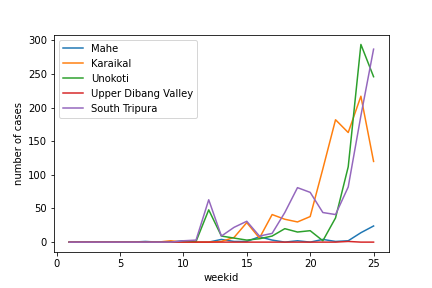
\includegraphics[width=\textwidth]{neighbor-coldspot.png}
    \caption{Biggest coldspots comparing with neighbor districts}
  \end{minipage}
  \hfill
  \begin{minipage}[b]{0.45\textwidth}
    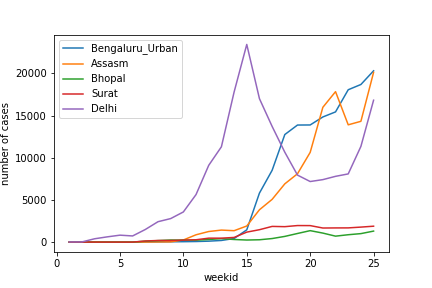
\includegraphics[width=\textwidth]{neighbor-hotspot.png}
    \caption{Biggest hotspots comparing with neighbor districts}
  \end{minipage}
\end{figure}




\begin{figure}[!tbp]
  \centering
  \begin{minipage}[b]{0.45\textwidth}
    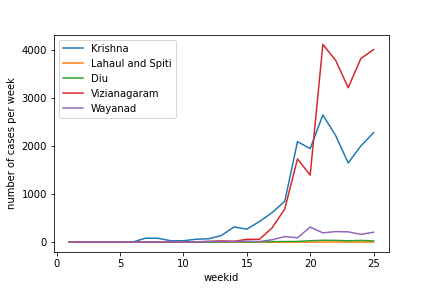
\includegraphics[width=\textwidth]{state-coldspot.png}
    \caption{Biggest coldspots comparing with state districts}
  \end{minipage}
  \hfill
  \begin{minipage}[b]{0.45\textwidth}
    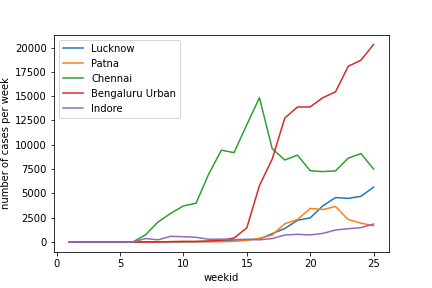
\includegraphics[width=\textwidth]{state-hotspot.png}
    \caption{Biggest hotspots comparing with state districts}
  \end{minipage}
\end{figure}


\section{Conclusion}
India is home to over 1.3 billion people. A total number of 4,086,973 confirmed COVID-19 cases, as observed in the time period of this study, though it looks extremely high at the surface of it, but it can be found reasonable when one takes into account its large population. The pattern of higher number of cases in an area with a high population  density can also be observed with the urban districts having high population like Pune, Mumbai Bangalore, being the most affected, and. districts with lesser population like Upper Dibang Valley, Kamla, being the least affected.

Due to the vast diversity of India, the number of infected people across various districts also varies greatly. Given limited resources, separate strategic approaches should be developed to tackle the pandemic in different districts based on its district wise infection rate. Therefore, a district-wise analysis is more beneficial to address the COVID-19 pandemic in India rather than nation-wise analysis, as it provides better insight. 


\end{document}
